\newpage\handout
{Drill Problems: Week 03-5}
{\textsc{Scholastic Aptitude Test (SAT)}}
{\href{https://creativecommons.org/licenses/by-nc-sa/4.0/}{CC BY-NC-SA 4.0 license}}
{Author: \BookAuthor}{Release: \generatedOn}
{SAT: Drill Problems (3-5)}
% Copyright & Disclaimer
\newcommand{\BookAuthor}{Jaehoon Song (Lecturer)}

\begin{center}
  \begin{minipage}{0.85\textwidth}
    {\small\textbf{Purpose and Usage:}}\\[0.2cm]
    {\footnotesize
    This material has been developed for internal training and educational 
    purposes at Hans edu LLC. It is intended for use within our organization 
    and should not be distributed, sold, or used for commercial purposes 
    outside of our educational programs.}\\[0.5cm]
    
    {\small\textbf{For Our Community:}}\\[0.2cm]
    {\footnotesize
    Students and staff are welcome to use this material in their studies and 
    teaching at Hans edu LLC. While we encourage active engagement with the 
    content, please respect that this is proprietary material. Any 
    reproduction or distribution outside of our organization's educational 
    activities is not permitted.}\\[0.5cm]
    
    {\small\textbf{Content and Attribution:}}\\[0.2cm]
    {\footnotesize
    This material represents our adaptation of various established mathematics 
    textbooks, reorganized and enhanced for our teaching context. While we've 
    added our own pedagogical improvements, we maintain proper attribution to 
    original sources. This work is shared under the Creative Commons 
    Attribution-NonCommercial-ShareAlike (CC BY-NC-SA) license, allowing 
    internal use and adaptation while respecting the original creators' rights.\\[0.2cm]
    \small Key Permissions under CC BY-NC-SA 4.0:
    \begin{itemize}
      \item credit the creator.
      \item no commercial use.
      \item new creations must carry the same license.
      \item copy and redistribute the material in any medium or format
      \item remix, transform, and build upon the material
    \end{itemize}}
    % Some content may be derived from sources under the CC0 1.0 Universal 
    % license, which allows for free use, modification, and distribution.}\\[0.5cm]
    {\small\textbf{Quality Assurance:}}\\[0.2cm]
    {\footnotesize
    We have carefully reviewed this material for accuracy and clarity. However, 
    as with any educational resource, we encourage critical engagement and 
    verification of concepts. If you notice any issues or have suggestions for 
    improvement, please bring them to our attention.}
  \end{minipage}
  \vspace{2cm} \\
  {\small © \the\year\ Hans edu LLC. All rights reserved.}\\[0.5cm]
  {\small Written by \BookAuthor}\\[1cm]
\end{center}

\newpage


\begin{enumerate}
  \item \textbf{Data Set Comparison} (10 points)\\
  \begin{center}
  \begin{tabular}{|l|l|l|}
  \hline
  Value & Data set A frequency & Data set B frequency \\
  \hline
  30 & 2 & 9 \\
  \hline
  34 & 4 & 7 \\
  \hline
  38 & 5 & 5 \\
  \hline
  42 & 7 & 4 \\
  \hline
  46 & 9 & 2 \\
  \hline
  \end{tabular}
  \end{center}

  Data set $A$ and data set $B$ each consist of 27 values. The table shows the frequencies of the values for each data set. Which of the following statements best compares the means of the two data sets?
  \begin{enumerate}[label=(\Alph*)]
    \item The mean of data set $A$ is greater than the mean of data set $B$.
    \item The mean of data set $A$ is less than the mean of data set $B$.
    \item The mean of data set $A$ is equal to the mean of data set $B$.
    \item There is not enough information to compare the means of the data sets.
  \end{enumerate}
  \begin{subanswer}
    % your answer here
  \end{subanswer}

  \item \textbf{Data Set Transformation} (10 points)\\
  A data set of 27 different numbers has a mean of 33 and a median of 33. A new data set is created by adding 7 to each number in the original data set that is greater than the median and subtracting 7 from each number in the original data set that is less than the median. Which of the following measures does NOT have the same value in both the original and new data sets?
  \begin{enumerate}[label=(\Alph*)]
    \item Median
    \item Mean
    \item Sum of the numbers
    \item Standard deviation
  \end{enumerate}
  \begin{subanswer}
    % your answer here
  \end{subanswer}

  \newpage

  \item \textbf{Median Calculation} (10 points)\\
  What is the median of the data shown?\\
  $$73,74,75,77,79,82,84,85,91$$
  \begin{subanswer}
    % your answer here
  \end{subanswer}

  \item \textbf{International Tourist Arrivals} (10 points)\\
  \begin{center}
  \begin{tabular}{|l|l|l|}
  \hline
  \multicolumn{3}{|c|}{International Tourist Arrivals, in millions} \\
  \hline
  Country & 2012 & 2013 \\
  \hline
  France & 83.0 & 84.7 \\
  \hline
  United States & 66.7 & 69.8 \\
  \hline
  Spain & 57.5 & 60.7 \\
  \hline
  China & 57.7 & 55.7 \\
  \hline
  Italy & 46.4 & 47.7 \\
  \hline
  Turkey & 35.7 & 37.8 \\
  \hline
  Germany & 30.4 & 31.5 \\
  \hline
  United Kingdom & 26.3 & 32.2 \\
  \hline
  Russia & 24.7 & 28.4 \\
  \hline
  \end{tabular}
  \end{center}

  The table above shows the number of international tourist arrivals, rounded to the nearest tenth of a million, to the top nine tourist destinations in both 2012 and 2013. Based on the information given in the table, how much greater, in millions, was the median number of international tourist arrivals to the top nine tourist destinations in 2013 than the median number in 2012, to the nearest tenth of a million?
  \begin{subanswer}
    % your answer here
  \end{subanswer}


  \newpage

  \item \textbf{Dot Plot Analysis} (10 points)\\
  The dot plots represent the distributions of values in data sets $A$ and $B$.
  \begin{center}
  \begin{tabular}{cc}
  Data Set A. & Data Set B. \\
  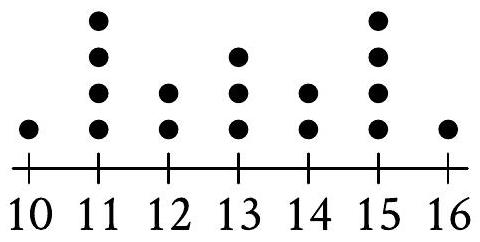
\includegraphics[width=0.23\textwidth]{images/2025_06_15_04f7426dc644de311e92g-15(1)} &
  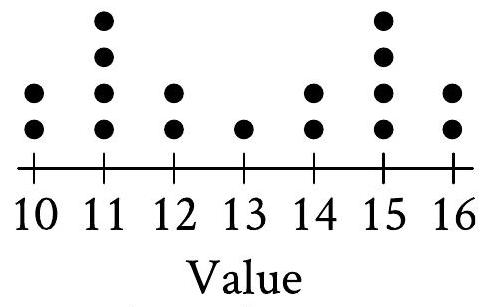
\includegraphics[width=0.23\textwidth]{images/2025_06_15_04f7426dc644de311e92g-15} \\
  \end{tabular}
  \end{center}
  Which of the following statements must be true?
  \begin{enumerate}[label=(\Alph*)]
    \item The median of data set $A$ is equal to the median of data set $B$.
    \item The standard deviation of data set $A$ is equal to the standard deviation of data set $B$.
  \end{enumerate}
  \begin{enumerate}[label=(\Alph*)]
    \item I only
    \item II only
    \item I and II
    \item Neither I nor II
  \end{enumerate}
  \begin{subanswer}
    % your answer here
  \end{subanswer}

  \newpage

  \item \textbf{Histogram Analysis} (10 points)\\
  \insertimage{0.40}{images/2025_06_15_04f7426dc644de311e92g-16}{reference attached}

  Two data sets of 23 integers each are summarized in the histograms shown. For each of the histograms, the first interval represents the frequency of integers greater than or equal to 10, but less than 20. The second interval represents the frequency of integers greater than or equal to 20, but less than 30, and so on. What is the smallest possible difference between the mean of data set $A$ and the mean of data set $B$?
  \begin{enumerate}[label=(\Alph*)]
    \item 0
    \item 1
    \item 10
    \item 23
  \end{enumerate}
  \begin{subanswer}
    % your answer here
  \end{subanswer}

  \item \textbf{Mean Calculation} (10 points)\\
  What is the mean of the data shown?\\
  $$2,9,14,23,32$$
  \begin{enumerate}[label=(\Alph*)]
    \item 14
    \item 16
    \item 17
    \item 32
  \end{enumerate}
  \begin{subanswer}
    % your answer here
  \end{subanswer}

  \newpage

  \item \textbf{Frequency Distribution} (10 points)\\
  \begin{center}
  \begin{tabular}{|c|c|}
  \hline
  Value & Frequency \\
  \hline
  1 & $a$ \\
  \hline
  2 & $2a$ \\
  \hline
  3 & $3a$ \\
  \hline
  4 & $2a$ \\
  \hline
  5 & $a$ \\
  \hline
  \end{tabular}
  \end{center}

  The frequency distribution above summarizes a set of data, where $a$ is a positive integer. How much greater is the mean of the set of data than the median?
  \begin{enumerate}[label=(\Alph*)]
    \item 0
    \item 1
    \item 2
    \item 3
  \end{enumerate}
  \begin{subanswer}
    % your answer here
  \end{subanswer}

  \item \textbf{Team Race Times} (10 points)\\
  Two different teams consisting of 10 members each ran in a race. Each member's completion time of the race was recorded. The mean of the completion times for each team was calculated and is shown below.\\
  Team A: 3.41 minutes\\
  Team B: 3.79 minutes\\
  Which of the following MUST be true?
  \begin{enumerate}[label=(\Alph*)]
    \item Every member of team $A$ completed the race in less time than any member of team $B$.
    \item The median time it took the members of team B to complete the race is greater than the median time it took the members of team A to complete the race.
    \item There is at least one member of team B who took more time to complete the race than some member of team A.
  \end{enumerate}
  \begin{enumerate}[label=(\Alph*)]
    \item III only
    \item I and III only
    \item II and III only
    \item I, II, and III
  \end{enumerate}
  \begin{subanswer}
    % your answer here
  \end{subanswer}

  \newpage

  \item \textbf{Basketball Score} (10 points)\\
  The mean score of 8 players in a basketball game was 14.5 points. If the highest individual score is removed, the mean score of the remaining 7 players becomes 12 points. What was the highest score?
  \begin{enumerate}[label=(\Alph*)]
    \item 20
    \item 24
    \item 32
    \item 36
  \end{enumerate}
  \begin{subanswer}
    % your answer here
  \end{subanswer}

  \item \textbf{Linear Model} (10 points)\\
  \insertimage{0.40}{images/2025_06_15_c6d1fe032100fbb48447g-11}{reference attached}

  Which of the following equations is the most appropriate linear model for the data shown in the scatterplot?
  \begin{enumerate}[label=(\Alph*)]
    \item $y=-1.9x-10.1$
    \item $y=-1.9x+10.1$
    \item $y=1.9x-10.1$
    \item $y=1.9x+10.1$
  \end{enumerate}
  \begin{subanswer}
    % your answer here
  \end{subanswer}

  \newpage

  \item \textbf{Stopping Distance} (10 points)\\
  A study was done to determine a new car's stopping distance when it was traveling at different speeds. The study was done on a dry road with good surface conditions. The results are shown below, along with the graph of a quadratic function that models the data.

  \insertimage{0.40}{images/2025_06_15_c6d1fe032100fbb48447g-12}{reference attached}

  According to the model, which of the following is the best estimate for the stopping distance, in feet, if the vehicle was traveling 55 miles per hour?
  \begin{enumerate}[label=(\Alph*)]
    \item 25
    \item 30
    \item 210
    \item 250
  \end{enumerate}
  \begin{subanswer}
    % your answer here
  \end{subanswer}


  \newpage

  \item \textbf{Temperature Change} (10 points)\\
  The scatterplot shows the temperature $y$, in ${ }^{\circ} \mathrm{F}$, recorded by a meteorologist at various times $x$, in days since June 1.

  \insertimage{0.40}{images/2025_06_15_c6d1fe032100fbb48447g-13}{reference attached}

  During which of the following time periods did the greatest increase in recorded temperature take place?
  \begin{enumerate}[label=(\Alph*)]
    \item From $x=6$ to $x=7$
    \item From $x=5$ to $x=6$
    \item From $x=2$ to $x=3$
    \item From $x=1$ to $x=2$
  \end{enumerate}
  \begin{subanswer}
    % your answer here
  \end{subanswer}


  \newpage

  \item \textbf{Line of Best Fit} (10 points)\\
  \insertimage{0.40}{images/2025_06_15_c6d1fe032100fbb48447g-14}{reference attached}
  Which of the following could be the equation for a line of best fit for the data shown in the scatterplot above?
  \begin{enumerate}[label=(\Alph*)]
    \item $y=3x+0.8$
    \item $y=0.8x+3$
    \item $y=-0.8x+3$
    \item $y=-3x+0.8$
  \end{enumerate}
  \begin{subanswer}
    % your answer here
  \end{subanswer}

  \newpage

  \item \textbf{Energy Generation} (10 points)\\
  The scatterplot below shows the amount of electric energy generated, in millions of megawatt-hours, by nuclear sources over a 10-year period.

  \insertimage{0.40}{images/2025_06_15_c6d1fe032100fbb48447g-15}{reference attached}
  Of the following equations, which best models the data in the scatterplot?
  \begin{enumerate}[label=(\Alph*)]
    \item $y=1.674x^{2}+19.76x-745.73$
    \item $y=-1.674x^{2}-19.76x-745.73$
    \item $y=1.674x^{2}+19.76x+745.73$
    \item $y=-1.674x^{2}+19.76x+745.73$
  \end{enumerate}
  \begin{subanswer}
    % your answer here
  \end{subanswer}

  \newpage

  \item \textbf{Beach Visitors} (10 points)\\
  \insertimage{0.40}{images/2025_06_15_c6d1fe032100fbb48447g-16}{reference attached}
  Each dot in the scatterplot above represents the temperature and the number of people who visited a beach in Lagos, Nigeria, on one of eleven different days. The line of best fit for the data is also shown. According to the line of best fit, what is the number of people, rounded to the nearest 10, predicted to visit this beach on a day with an average temperature of $32^{\circ} \mathrm{C}$?
  \begin{enumerate}[label=(\Alph*)]
    \item 120
    \item 130
    \item 140
    \item 150
  \end{enumerate}
  \begin{subanswer}
    % your answer here
  \end{subanswer}


  \newpage

  \item \textbf{Chipmunk Population} (10 points)\\
  The line graph shows the estimated number of chipmunks in a state park on April 1 of each year from 1989 to 1999.

  \insertimage{0.40}{images/2025_06_15_c6d1fe032100fbb48447g-17}{reference attached}

  Based on the line graph, in which year was the estimated number of chipmunks in the state park the greatest?
  \begin{enumerate}[label=(\Alph*)]
    \item 1989
    \item 1994
    \item 1995
    \item 1998
  \end{enumerate}
  \begin{subanswer}
    % your answer here
  \end{subanswer}

  \item \textbf{Nonlinear Relationship} (10 points)\\
  In which of the following tables is the relationship between the values of $x$ and their corresponding $y$-values nonlinear?
  \begin{enumerate}[label=(\Alph*)]
    \item 
    \begin{center}
    \begin{tabular}{|r|r|r|r|r|}
    \hline
    $x$ & 1 & 2 & 3 & 4 \\
    \hline
    $y$ & 8 & 11 & 14 & 17 \\
    \hline
    \end{tabular}
    \end{center}

    \item 
    \begin{center}
    \begin{tabular}{|l|l|l|r|r|}
    \hline
    $x$ & 1 & 2 & 3 & 4 \\
    \hline
    $y$ & 4 & 8 & 12 & 16 \\
    \hline
    \end{tabular}
    \end{center}

    \item 
    \begin{center}
    \begin{tabular}{|r|r|r|r|r|}
    \hline
    $x$ & 1 & 2 & 3 & 4 \\
    \hline
    $y$ & 8 & 13 & 18 & 23 \\
    \hline
    \end{tabular}
    \end{center}

    \item 
    \begin{center}
    \begin{tabular}{|r|r|r|r|r|}
    \hline
    $x$ & 1 & 2 & 3 & 4 \\
    \hline
    $y$ & 6 & 12 & 24 & 48 \\
    \hline
    \end{tabular}
    \end{center}
  \end{enumerate}
  \begin{subanswer}
    % your answer here
  \end{subanswer}


  \newpage

  \item \textbf{Braking Distance} (10 points)\\
  \insertimage{0.40}{images/2025_06_15_c6d1fe032100fbb48447g-19}{reference attached}

  The graph above shows the relationship between the speed of a particular car, in miles per hour, and its corresponding braking distance, in feet. Approximately how many feet greater will the car's braking distance be when the car is traveling at 50 miles per hour than when the car is traveling at 30 miles per hour?
  \begin{enumerate}[label=(\Alph*)]
    \item 75
    \item 125
    \item 175
    \item 250
  \end{enumerate}
  \begin{subanswer}
    % your answer here
  \end{subanswer}

  \newpage

  \item \textbf{Line of Best Fit} (10 points)\\
  \insertimage{0.40}{images/2025_06_15_c6d1fe032100fbb48447g-20}{reference attached}

  Which of the following could be an equation for a line of best fit for the data in the scatterplot?
  \begin{enumerate}[label=(\Alph*)]
    \item $y=-x+6$
    \item $y=-x-6$
    \item $y=6x+1$
    \item $y=6x-1$
  \end{enumerate}
  \begin{subanswer}
    % your answer here
  \end{subanswer}

  \item \textbf{Wind Turbine} (10 points)\\
  A wind turbine completes 900 revolutions in 50 minutes. At this rate, how many revolutions per minute does this turbine complete?
  \begin{enumerate}[label=(\Alph*)]
    \item 18
    \item 850
    \item 950
    \item 1,400
  \end{enumerate}
  \begin{subanswer}
    % your answer here
  \end{subanswer}

  \item \textbf{Constant Ratio} (10 points)\\
  \begin{center}
  \begin{tabular}{|c|c|}
  \hline
  $x$ & $y$ \\
  \hline
  1 & 4 \\
  \hline
  3 & 12 \\
  \hline
  5 & 20 \\
  \hline
  40 & $k$ \\
  \hline
  \end{tabular}
  \end{center}

  In the table above, the ratio of $y$ to $x$ for each ordered pair is constant. What is the value of $k$?
  \begin{enumerate}[label=(\Alph*)]
    \item 28
    \item 36
    \item 80
    \item 160
  \end{enumerate}
  \begin{subanswer}
    % your answer here
  \end{subanswer}

  \item \textbf{Tree Growth} (10 points)\\
  \begin{center}
  \begin{tabular}{|c|c|}
  \hline
  Species of tree & Growth factor \\
  \hline
  Red maple & 4.5 \\
  \hline
  River birch & 3.5 \\
  \hline
  Cottonwood & 2.0 \\
  \hline
  Black walnut & 4.5 \\
  \hline
  White birch & 5.0 \\
  \hline
  American elm & 4.0 \\
  \hline
  Pin oak & 3.0 \\
  \hline
  Shagbark hickory & 7.5 \\
  \hline
  \end{tabular}
  \end{center}

  One method of calculating the approximate age, in years, of a tree of a particular species is to multiply the diameter of the tree, in inches, by a constant called the growth factor for that species. The table above gives the growth factors for eight species of trees. If a white birch tree and a pin oak tree each now have a diameter of 1 foot, which of the following will be closest to the difference, in inches, of their diameters 10 years from now? (1 foot = 12 inches)
  \begin{enumerate}[label=(\Alph*)]
    \item 1.0
    \item 1.2
    \item 1.3
    \item 1.4
  \end{enumerate}
  \begin{subanswer}
    % your answer here
  \end{subanswer}

  \item \textbf{Ratio} (10 points)\\
  The ratio of $t$ to $u$ is 1 to 2, and $t=10$.\\
  What is the value of $u$?
  \begin{enumerate}[label=(\Alph*)]
    \item 2
    \item 5
    \item 10
    \item 20
  \end{enumerate}
  \begin{subanswer}
    % your answer here
  \end{subanswer}

  \item \textbf{Depth Conversion} (10 points)\\
  A special camera is used for underwater ocean research. When the camera is at a depth of 58 fathoms, what is the camera's depth in feet? (1 fathom = 6 feet)
  \begin{subanswer}
    % your answer here
  \end{subanswer}

  \item \textbf{Oak Density} (10 points)\\
  A sample of oak has a density of 807 kilograms per cubic meter. The sample is in the shape of a cube, where each edge has a length of 0.90 meters. To the nearest whole number, what is the mass, in kilograms, of this sample?
  \begin{enumerate}[label=(\Alph*)]
    \item 588
    \item 726
    \item 897
    \item 1,107
  \end{enumerate}
  \begin{subanswer}
    % your answer here
  \end{subanswer}

  \item \textbf{Average Speed} (10 points)\\
  On April 18, 1775, Paul Revere set off on his midnight ride from Charlestown to Lexington. 
  If he had ridden straight to Lexington without stopping, he would have traveled 11 miles 
  in 26 minutes. In such a ride, what would the average speed of his horse have been, to 
  the nearest tenth of a mile per \underbar{hour}?
  \begin{subanswer}
    % your answer here
  \end{subanswer}

  \newpage

  \item \textbf{Length Conversion} (10 points)\\
  How many yards are equivalent to 612 inches? (1 yard = 36 inches)
  \begin{enumerate}[label=(\Alph*)]
    \item 0.059
    \item 17
    \item 576
    \item 22,032
  \end{enumerate}
  \begin{subanswer}
    % your answer here
  \end{subanswer}

  \item \textbf{Rectangle Ratio} (10 points)\\
  Rectangle $A$ has length 15 and width $w$. Rectangle $B$ has length 20 and the same length-to-width ratio as rectangle $A$. What is the width of rectangle $B$ in terms of $w$?
  \begin{enumerate}[label=(\Alph*)]
    \item $\frac{4}{3}w$
    \item $w+5$
    \item $\frac{3}{4}w$
    \item $w-5$
  \end{enumerate}
  \begin{subanswer}
    % your answer here
  \end{subanswer}

  \item \textbf{Card Ratio} (10 points)\\
  Shaquan has 7 red cards and 28 blue cards. What is the ratio of red cards to blue cards that Shaquan has?
  \begin{enumerate}[label=(\Alph*)]
    \item 1 to 4
    \item 4 to 1
    \item 1 to 7
    \item 7 to 1
  \end{enumerate}
  \begin{subanswer}
    % your answer here
  \end{subanswer}

  \item \textbf{Plant Growth} (10 points)\\
  Last year, Cedric had 35 plants in his garden. This year, the number of 
  plants in Cedric's garden is $60\%$ greater than the number of plants in 
  his garden last year. How many plants does Cedric have in his garden this year?
  \begin{subanswer}
    % your answer here
  \end{subanswer}

  \newpage

  \item \textbf{Percentage} (10 points)\\
  What is $23\%$ of 100?
  \begin{enumerate}[label=(\Alph*)]
    \item 23
    \item 46
    \item 77
    \item 123
  \end{enumerate}
  \begin{subanswer}
    % your answer here
  \end{subanswer}

  \item \textbf{Percentage Increase} (10 points)\\
  Which expression represents the result of increasing a positive quantity $w$ by $43\%$?
  \begin{enumerate}[label=(\Alph*)]
    \item $1.43w$
    \item $0.57w$
    \item $43w$
    \item $0.43w$
  \end{enumerate}
  \begin{subanswer}
    % your answer here
  \end{subanswer}

  \item \textbf{Population Growth} (10 points)\\
  The population of City A increased by $7\%$ from 2015 to 2016. If the 2016 population is $k$ times the 2015 population, what is the value of $k$?
  \begin{enumerate}[label=(\Alph*)]
    \item 0.07
    \item 0.7
    \item 1.07
    \item 1.7
  \end{enumerate}
  \begin{subanswer}
    % your answer here
  \end{subanswer}

  \item \textbf{Percentage} (10 points)\\
  What is $10\%$ of 470?
  \begin{enumerate}[label=(\Alph*)]
    \item 37
    \item 47
    \item 423
    \item 460
  \end{enumerate}
  \begin{subanswer}
    % your answer here
  \end{subanswer}

  \item \textbf{Percentage Increase} (10 points)\\
  Which of the following represents the result of increasing the quantity $x$ by $9\%$, where $x>0$?
  \begin{enumerate}[label=(\Alph*)]
    \item $1.09x$
    \item $0.09x$
    \item $x+9$
    \item $x+0.09$
  \end{enumerate}
  \begin{subanswer}
    % your answer here
  \end{subanswer}

  \item \textbf{Percentage Greater} (10 points)\\
  The number $k$ is $36\%$ greater than 50. If $k$ is the product of 50 and $r$, what is the value of $r$?
  \begin{enumerate}[label=(\Alph*)]
    \item 36
    \item 3.6
    \item 1.36
    \item 0.36
  \end{enumerate}
  \begin{subanswer}
    % your answer here
  \end{subanswer}

  \item \textbf{Percentage Comparison} (10 points)\\
  The number $a$ is $70\%$ less than the positive number $b$. The number $c$ is $80\%$ greater than $a$. The number $c$ is how many times $b$?
  \begin{subanswer}
    % your answer here
  \end{subanswer}

  \item \textbf{Percentage Greater} (10 points)\\
  210 is $p\%$ greater than 30. What is the value of $p$?
  \begin{subanswer}
    % your answer here
  \end{subanswer}

  \item \textbf{Percentage Greater} (10 points)\\
  The value of $z$ is 1.13 times 100. The value of $z$ is what percent greater than 100?
  \begin{enumerate}[label=(\Alph*)]
    \item 11.3
    \item 13
    \item 130
    \item 213
  \end{enumerate}
  \begin{subanswer}
    % your answer here
  \end{subanswer}

  \item \textbf{Survey Analysis} (10 points)\\
  A city has 50 city council members. A reporter polled a random sample of 20 city council members and found that 6 of those polled supported a specific bill. Based on the sample, which of the following is the best estimate of the number of city council members in the city who support the bill?
  \begin{enumerate}[label=(\Alph*)]
    \item 6
    \item 9
    \item 15
    \item 30
  \end{enumerate}
  \begin{subanswer}
    % your answer here
  \end{subanswer}

  \item \textbf{Fish Weight Study} (10 points)\\
  A study was done on the weights of different types of fish in a pond. A random sample of fish were caught and marked in order to ensure that none were weighed more than once. The sample contained 150 largemouth bass, of which $30\%$ weighed more than 2 pounds. Which of the following conclusions is best supported by the sample data?
  \begin{enumerate}[label=(\Alph*)]
    \item The majority of all fish in the pond weigh less than 2 pounds.
    \item The average weight of all fish in the pond is approximately 2 pounds.
    \item Approximately $30\%$ of all fish in the pond weigh more than 2 pounds.
    \item Approximately $30\%$ of all largemouth bass in the pond weigh more than 2 pounds.
  \end{enumerate}
  \begin{subanswer}
    % your answer here
  \end{subanswer}

  \item \textbf{Hiking Survey} (10 points)\\
  A park ranger asked a random sample of visitors how far they hiked during their visit. Based on the responses, the estimated mean was found to be 4.5 miles, with an associated margin of error of 0.5 miles. Which of the following is the best conclusion from these data?
  \begin{enumerate}[label=(\Alph*)]
    \item It is likely that all visitors hiked between 4 and 5 miles.
    \item It is likely that most visitors hiked exactly 4.5 miles.
    \item It is not possible that any visitor hiked less than 3 miles.
    \item It is plausible that the mean distance hiked for all visitors is between 4 and 5 miles.
  \end{enumerate}
  \begin{subanswer}
    % your answer here
  \end{subanswer}

  \newpage

  \item \textbf{Kitten Characteristics} (10 points)\\
  \begin{center}
  \begin{tabular}{|c|c|c|c|}
  \hline
  Coat color & \multicolumn{3}{|c|}{Eye color} \\
  \hline
  & Deep blue & Light brown & Total \\
  \hline
  Cream-tortoiseshell & 16 & 16 & 32 \\
  \hline
  Chocolate & 12 & 4 & 16 \\
  \hline
  Total & 28 & 20 & 48 \\
  \hline
  \end{tabular}
  \end{center}

  The data on the coat color and eye color for 48 Himalayan kittens available for adoption were collected and summarized in the table above. What fraction of the chocolate-colored kittens has deep blue eyes?
  \begin{enumerate}[label=(\Alph*)]
    \item $\frac{12}{48}$
    \item $\frac{12}{28}$
    \item $\frac{16}{32}$
    \item $\frac{12}{16}$
  \end{enumerate}
  \begin{subanswer}
    % your answer here
  \end{subanswer}

  \item \textbf{Internship Data} (10 points)\\
  \begin{center}
  \begin{tabular}{|l|c|c|c|c|c|}
  \hline
  High school & \multicolumn{5}{|c|}{Year} \\
  \hline
  & 2008 & 2009 & 2010 & 2011 & 2012 \\
  \hline
  Foothill & 87 & 80 & 75 & 76 & 70 \\
  \hline
  Valley & 44 & 54 & 65 & 76 & 82 \\
  \hline
  Total & 131 & 134 & 140 & 152 & 152 \\
  \hline
  \end{tabular}
  \end{center}

  The table above shows the number of students from two different high schools who completed summer internships in each of five years. No student attended both schools. Of the students who completed a summer internship in 2010, which of the following represents the fraction of students who were from Valley High School?
  \begin{enumerate}[label=(\Alph*)]
    \item $\frac{10}{140}$
    \item $\frac{65}{140}$
    \item $\frac{75}{140}$
    \item $\frac{65}{75}$
  \end{enumerate}
  \begin{subanswer}
    % your answer here
  \end{subanswer}

  \newpage

  \item \textbf{Singing Lessons} (10 points)\\
  \begin{center}
  \begin{tabular}{|c|c|}
  \hline
  Voice type & Number of singers \\
  \hline
  Countertenor & 4 \\
  \hline
  Tenor & 6 \\
  \hline
  Baritone & 10 \\
  \hline
  Bass & 5 \\
  \hline
  \end{tabular}
  \end{center}

  A total of 25 men registered for singing lessons. The frequency table shows how many of these singers have certain voice types. If one of these singers is selected at random, what is the probability he is a baritone?
  \begin{enumerate}[label=(\Alph*)]
    \item 0.10
    \item 0.40
    \item 0.60
    \item 0.67
  \end{enumerate}
  \begin{subanswer}
    % your answer here
  \end{subanswer}

  \item \textbf{Sports Survey} (10 points)\\
  A survey taken by 1,000 students at a school asked whether they played school sports. The table below summarizes all 1,000 responses from the students surveyed.

  \begin{center}
  \begin{tabular}{|l|c|c|}
  \hline
  & Males & Females \\
  \hline
  Play a school sport & 312 & 220 \\
  \hline
  Do not play a school sport & $?$ & 216 \\
  \hline
  \end{tabular}
  \end{center}

  How many of the males surveyed responded that they do not play a school sport?
  \begin{enumerate}[label=(\Alph*)]
    \item 109
    \item 252
    \item 468
    \item 688
  \end{enumerate}
  \begin{subanswer}
    % your answer here
  \end{subanswer}

  \newpage

  \item \textbf{Blood Type Distribution} (10 points)\\
  \begin{center}
  \begin{tabular}{|c|c|c|c|c|}
  \hline
  & \multicolumn{4}{|c|}{Blood type} \\
  \hline
  Rhesus factor & A & B & AB & O \\
  \hline
  + & 33 & 9 & 3 & 37 \\
  \hline
  - & 7 & 2 & 1 & $x$ \\
  \hline
  \end{tabular}
  \end{center}

  Human blood can be classified into four common blood types-A, B, AB, and O. It is also characterized by the presence $(+)$ or absence $(-)$ of the rhesus factor. The table above shows the distribution of blood type and rhesus factor for a group of people. If one of these people who is rhesus negative $(-)$ is chosen at random, the probability that the person has blood type $B$ is $\frac{1}{9}$. What is the value of $x$?
  \begin{subanswer}
    % your answer here
  \end{subanswer}

  \item \textbf{Survey Generalization} (10 points)\\
  A survey was conducted using a sample of history professors selected at random from the California State Universities. The professors surveyed were asked to name the publishers of their current texts. What is the largest population to which the results of the survey can be generalized?
  \begin{enumerate}[label=(\Alph*)]
    \item All professors in the United States
    \item All history professors in the United States
    \item All history professors at all California State Universities
    \item All professors at all California State Universities
  \end{enumerate}
  \begin{subanswer}
    % your answer here
  \end{subanswer}

  \item \textbf{Dog Park Survey} (10 points)\\
  The members of a city council wanted to assess the opinions of all city residents about converting an open field into a dog park. The council surveyed a sample of 500 city residents who own dogs. The survey showed that the majority of those sampled were in favor of the dog park. Which of the following is true about the city council's survey?
  \begin{enumerate}[label=(\Alph*)]
    \item It shows that the majority of city residents are in favor of the dog park.
    \item The survey sample should have included more residents who are dog owners.
    \item The survey sample should have consisted entirely of residents who do not own dogs.
    \item The survey sample is biased because it is not representative of all city residents.
  \end{enumerate}
  \begin{subanswer}
    % your answer here
  \end{subanswer}
\end{enumerate}

